
Let
\begin{align}
\textbf{L}=\myvec{0 \\ l},
\textbf{M}=\myvec{0 \\ 0} ,
\textbf{N}=\myvec{3 \\ 0}
\end{align}
From the given information, 
\begin{align}
\norm{\vec{N}-\vec{M}}^2 &= \norm{\vec{N}}^2  = 3^2 =9
\\
\norm{\vec{L}-\vec{M}}^2 &= \norm{\vec{L}}^2 =l^2
\\
\norm{\vec{L}-\vec{N}}^2 &=5^2=25
\end{align}
which can  be expressed as
\begin{align}
\norm{\vec{L}-\vec{N}}^2 &= ({\vec{L}-\vec{N}})^T({\vec{L}-\vec{N}})
% \\
% &= \vec{L}^T\vec{L}+\vec{N}^T\vec{N}-\vec{L}^T\vec{N} - \vec{L}^T\vec{L}
\\
&= \norm{\vec{L}}^2 + \norm{\vec{N}}^2 - 2\vec{L}^T\vec{N}
% \\
% &= \norm{\vec{L}}^2 + \norm{\vec{N}}^2-2.0
% \\
% &= l^2 + 3^2
\\
\implies l^2+9 &= 25
\\
\text{or, } l &= \pm 4
\end{align}
% But we know LN=5 
% \begin{align}
% \norm{{\vec{L}-\vec{N}}}^2=5^2=25
% \\
% l^2+9=25
% \\
% l^2=25-9
% \\
% l^2=16
% \\
% l=\pm4
% \end{align}

For  $l$=4, $\triangle LMN$  is plotted in the first quadrant in  Fig. \ref{constr/23/fig:Right Angle}.

%\numberwithin{figure}{section}
\begin{figure}[ht]
    \centering
    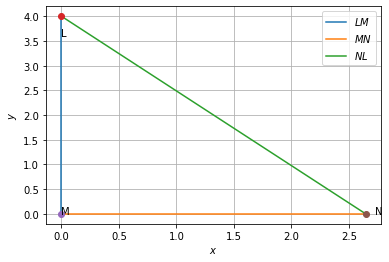
\includegraphics[width=\columnwidth]{solutions/23/RIGHT_TRIANGLE.png}
    \caption{}
    \label{constr/23/fig:Right Angle}
\end{figure}
























